%%%%%%%%%%%%%%%%%%%%%%%%%%%%%%%%%%%%%%%%%
% Short Sectioned Assignment LaTeX Template Version 1.0 (5/5/12)
% This template has been downloaded from: http://www.LaTeXTemplates.com
% Original author:  Frits Wenneker (http://www.howtotex.com)
% License: CC BY-NC-SA 3.0 (http://creativecommons.org/licenses/by-nc-sa/3.0/)
%%%%%%%%%%%%%%%%%%%%%%%%%%%%%%%%%%%%%%%%%

%----------------------------------------------------------------------------------------
%	PACKAGES AND OTHER DOCUMENT CONFIGURATIONS
%----------------------------------------------------------------------------------------

\documentclass[paper=a4, fontsize=11pt]{scrartcl} % A4 paper and 11pt font size

% ---- Entrada y salida de texto -----

\usepackage[T1]{fontenc} % Use 8-bit encoding that has 256 glyphs
\usepackage[utf8]{inputenc}
%\usepackage{fourier} % Use the Adobe Utopia font for the document - comment this line to return to the LaTeX default

% ---- Idioma --------

\usepackage[spanish, es-tabla]{babel} % Selecciona el español para palabras introducidas automáticamente, p.ej. "septiembre" en la fecha y especifica que se use la palabra Tabla en vez de Cuadro

% ---- Otros paquetes ----

\usepackage{url} % ,href} %para incluir URLs e hipervínculos dentro del texto (aunque hay que instalar href)
\usepackage{amsmath,amsfonts,amsthm} % Math packages
%\usepackage{graphics,graphicx, floatrow} %para incluir imágenes y notas en las imágenes
\usepackage{graphics,graphicx, float} %para incluir imágenes y colocarlas

% Para hacer tablas comlejas
%\usepackage{multirow}
%\usepackage{threeparttable}

%\usepackage{sectsty} % Allows customizing section commands
%\allsectionsfont{\centering \normalfont\scshape} % Make all sections centered, the default font and small caps

\usepackage{fancyhdr} % Custom headers and footers
\pagestyle{fancyplain} % Makes all pages in the document conform to the custom headers and footers
\fancyhead{} % No page header - if you want one, create it in the same way as the footers below
\fancyfoot[L]{} % Empty left footer
\fancyfoot[C]{} % Empty center footer
\fancyfoot[R]{\thepage} % Page numbering for right footer
\renewcommand{\headrulewidth}{0pt} % Remove header underlines
\renewcommand{\footrulewidth}{0pt} % Remove footer underlines
\setlength{\headheight}{13.6pt} % Customize the height of the header

\numberwithin{equation}{section} % Number equations within sections (i.e. 1.1, 1.2, 2.1, 2.2 instead of 1, 2, 3, 4)
\numberwithin{figure}{section} % Number figures within sections (i.e. 1.1, 1.2, 2.1, 2.2 instead of 1, 2, 3, 4)
\numberwithin{table}{section} % Number tables within sections (i.e. 1.1, 1.2, 2.1, 2.2 instead of 1, 2, 3, 4)

\setlength\parindent{0pt} % Removes all indentation from paragraphs - comment this line for an assignment with lots of text

\newcommand{\horrule}[1]{\rule{\linewidth}{#1}} % Create horizontal rule command with 1 argument of height

\graphicspath{ {./images/} }
\usepackage{subcaption}
\usepackage{hyperref}
%\usepackage{soul}


%----------------------------------------------------------------------------------------
%	TÍTULO Y DATOS DEL ALUMNO
%----------------------------------------------------------------------------------------

\title{	
\normalfont \normalsize 
\textsc{\textbf{Aprendizaje no supervisado y detección de anomalías (2020)} \\ Máster Oficial Universitario en Ciencia de Datos e Ingeniería de Computadores \\ Universidad de Granada} \\ [25pt] % Your university, school and/or department name(s)
\horrule{0.5pt} \\[0.4cm] % Thin top horizontal rule
\huge Trabajo Final de Reglas de Asociación \\ % The assignment title
\horrule{2pt} \\[0.5cm] % Thick bottom horizontal rule
}

\author{Luis Balderas Ruiz \\ \texttt{luisbalderas@correo.ugr.es}} 
 % Nombre y apellidos 


\date{\normalsize\today} % Incluye la fecha actual

%----------------------------------------------------------------------------------------
% DOCUMENTO
%----------------------------------------------------------------------------------------

\begin{document}

\maketitle % Muestra el Título

\newpage %inserta un salto de página

\tableofcontents % para generar el índice de contenidos

\listoffigures

\listoftables

\newpage

%\begin{figure}[H] %con el [H] le obligamos a situar aquí la figura
%	\centering
%	\includegraphics[scale=0.6]{f1.png}  %el parámetro scale permite agrandar o achicar la imagen. En el nombre de archivo puede especificar directorios
%	\caption{Progresión de la imagen de f en cada iteración} 
%	\label{fig:f1}
%\end{figure}
%----------------------------------------------------------------------------------------
%	Introducción
%----------------------------------------------------------------------------------------

\section{Introducción}

En el presente documento se desarrolla el contenido del trabajo de Reglas de Asociación de la asignatura Aprendizaje no supervisado y Detección de Anomalías. Dicho trabajo se centra en el conjunto de datos \textit{Basketball} del repositorio \textit{http://keel.es/}, formado por 96 instancias, 3 variables reales (assists-per-minuteReal, time-playedReal y points-per-minuteReal) y 2 enteras (heightInteger y ageInteger). En primer lugar, me ocupo de hacer un pequeño análisis exploratorio de datos y a comentar las modificaciones hechas sobre el dataset previa aplicación de los algoritmos de minería.

\subsection{Exploración de datos}

Como se ha comentado, tenemos cinco variables que reflejan las estadísticas de 96 jugadores en ciertos partidos de baloncesto:  \textit{heightInteger}, referida a la altura del jugador; \textit{ageInteger}, referida a la edad del jugador;  \textit{time-playedReal} referida al número de minutos jugados en el partido; \textit{assists-per-minuteReal} que muestra el número de asistencias por minuto; y \textit{points-per-minuteReal} que se refiere al número de puntos por minuto. Para ganar interpretabilidad, y suponiendo que se trata de partidos en el ámbito de baloncesto FIBA (40 minutos por partido), genero dos nuevas variables llamadas \textit{points} y \textit{assists} que reflejan los puntos y asistencias por partido (multiplicando las anteriores por 40). A continuación, estudiamos con más detalle las variables

\subsubsection{Resumen estadístico}

Presento un resumen estadístico de las variables. Además, en el script incluyo la construcción de histogramas para cada una de ellas y se ve que las distribuciones son irregulares y en ningún caso normales.

\begin{figure}[H] %con el [H] le obligamos a situar aquí la figura
	\centering
	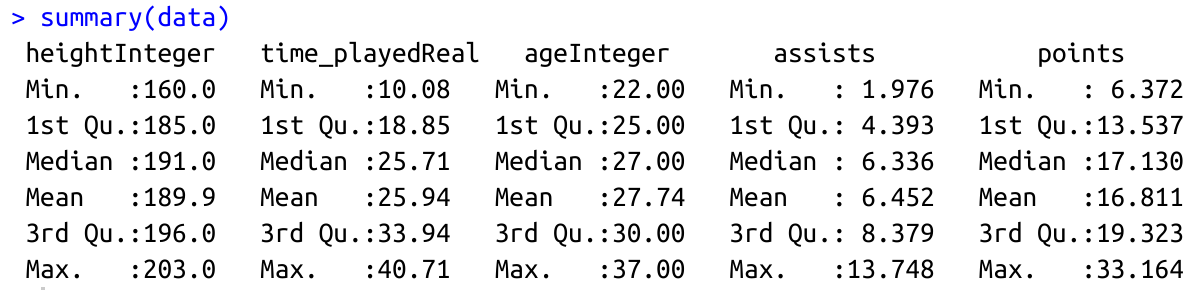
\includegraphics[scale=0.3]{summary.png}  %el parámetro scale permite agrandar o achicar la imagen. En el nombre de archivo puede especificar directorios
	\caption{Resumen estadístico de las variables} 
	\label{fig:summary}
\end{figure}

\subsection{Esquema de trabajo}

Presento tres aproximaciones en la búsqueda de reglas de asociación interesantes. La primera de ellas se basa en la forma clásica: defino una partición de datos, genero transacciones y aplico el algoritmo Apriori para encontrar itemsets frecuentes y reglas de asociación. Ante la problemática de definir una partición correcta, en la segunda aproximación aplico MOPNAR para encontrar la partición óptima según el algoritmo. Por último, contemplo el caso en que la división del conjunto de datos no sea una partición sino un recubrimiento, es decir, la intersección de los intervalos no es vacía. Así, puedo generar reglas afirmativas y negativas (como en el caso de MOPNAR) y estudiar conjuntos de reglas con las pautas dadas en el curso. 

\section{Primera aproximación: Partición de datos y búsqueda de reglas con Apriori}

Como se ha comentado, esta primera aproximación es la tradicional, es decir, con conocimiento de un 'experto' (el mío, como jugador y aficionado de baloncesto), realizo una partición de los datos, ya que estos vienen expresados de forma numérica y los algoritmos clásicos de reglas de asociación (Apriori) necesitan de variables categóricas. Presento a continuación las distintas categorías surgidas de cada variable:

\begin{table}[H]
	\centering
	\begin{tabular}{|c|c|c|c|c|c|}
		\hline
		\multicolumn{6}{|c|}{\textbf{ALTURA}}                                                         \\ \hline
		\textbf{Rangos (cm)} & ${[}159,175{]}$ & $(175.182{]}$ & $(182,190{]}$  & $(190,198{]}$ & $(198,203{]}$ \\ \hline
		\textbf{Categorías}  & Muy bajo      & Bajo        & Media altura & Alto        & Muy alto    \\ \hline
	\end{tabular}
	\caption{Tabla de transformación. Altura}
\end{table}

\begin{table}[H]
	\centering
	\begin{tabular}{|c|c|c|c|c|c|}
		\hline
		\multicolumn{6}{|c|}{\textbf{ASISTENCIAS}}                                                                                                                                                                                                                                                                                              \\ \hline
		\textbf{Rangos (por partido)} & $[1.97,3.5]$                                             & $(3.5,5.7]$                                               & $(5.7,7.2]$                                                & $(7.2,9]$                                                 & $(9,13.8]$                                              \\ \hline
		\textbf{Categorías}           & \begin{tabular}[c]{@{}c@{}}Mal \\ asistente\end{tabular} & \begin{tabular}[c]{@{}c@{}}Poco \\ asistente\end{tabular} & \begin{tabular}[c]{@{}c@{}}Asistente \\ medio\end{tabular} & \begin{tabular}[c]{@{}c@{}}Gran\\  asistente\end{tabular} & \begin{tabular}[c]{@{}c@{}}Pasador \\ nato\end{tabular} \\ \hline
	\end{tabular}
	\caption{Tabla de transformación. Asistencias}
\end{table}

\begin{table}[H]
	\centering
	\begin{tabular}{|c|c|c|c|c|c|}
		\hline
		\multicolumn{6}{|c|}{\textbf{EDAD}}                                                    \\ \hline
		\textbf{Rangos (años)} & $[21,25]$ & $(25,29]$ & $(29,32]$ & $(32,34]$     & $(34,37]$ \\ \hline
		\textbf{Categorías}    & Rookie    & Sophomore & Senior    & Experimentado & Coach     \\ \hline
	\end{tabular}
	\caption{Tabla de transformación. Edad}
\end{table}

\begin{table}[H]
	\centering
	\begin{tabular}{|c|c|c|c|c|c|}
		\hline
		\multicolumn{6}{|c|}{\textbf{TIEMPO DE JUEGO}}                                                                                                \\ \hline
		\textbf{Rangos (en minutos)} & $[10,16.5]$ & $(16.5,22.3]$ & $(22.3,27.9]$                                          & $(27.9,34]$ & $(34,41]$ \\ \hline
		\textbf{Categorías}          & Recambio    & Suplente      & \begin{tabular}[c]{@{}c@{}}Sexto\\ hombre\end{tabular} & Titular     & Estrella  \\ \hline
	\end{tabular}
	\caption{Tabla de transformación. Tiempo de juego}
\end{table}

\begin{table}[H]
	\centering
	\begin{tabular}{|c|c|c|c|c|c|}
		\hline
		\multicolumn{6}{|c|}{\textbf{PUNTUACIÓN}}                                                                                                                                        \\ \hline
		\textbf{Rangos}     & $[6,12]$                                                 & $(15,15]$ & $(15,22]$ & $(22,27]$    & $(27,34]$                                                \\ \hline
		\textbf{Categorías} & \begin{tabular}[c]{@{}c@{}}Baja\\ anotación\end{tabular} & Discreto  & Anotador  & Determinante & \begin{tabular}[c]{@{}c@{}}Amo\\ del parqué\end{tabular} \\ \hline
	\end{tabular}
	\caption{Tabla de transformación. Puntuación}
\end{table}

Con esta partición, se generan 96 transacciones cuyos itemsets más frecuentes son heightInteger=Altos (51), points=Anotador (51), ageInteger=Sophomore (36), heightInteger=Media altura (33) y assists=Poco asistente (33). Veamos el gráfico de itemsets:

\begin{figure}[H] %con el [H] le obligamos a situar aquí la figura
	\centering
	\includegraphics[scale=1.3]{ifp.png}  %el parámetro scale permite agrandar o achicar la imagen. En el nombre de archivo puede especificar directorios
	\caption{Gráfico de itemsets} 
	\label{fig:ifp}
\end{figure}

El objetivo que me he planteado sobre este conjunto de datos es saber qué aportan los jugadores en el partido o, en otras palabras, por qué el entrenador los mantiene más o menos minutos en pista. Por tanto, en lo que sigue me preguntó, en cada situación, qué claves a mi juicio hacen que un jugador pueda ser determinante. Para cada variable, estudiaré subcasos que puedan ser interesantes y presento las reglas asociadas junto con sus medidas.

\subsection{Reglas sobre altura}

\subsubsection{Altura: Bajos}
¿Qué hace que un jugador bajo sea importante en el equipo de baloncesto? Encontramos dos reglas que a mi juicio son interesantes:
$$\{ageInteger = Senior\} \Rightarrow \{assists = \text{Gran asistente}\}$$
con soporte 0.4, confianza 1 y Lift 2.5. Es decir, si un jugador es bajo y además tiene una cierta experiencia, será un gran asistente, y ese es su valor fundamental. Además, encontramos la relación recíproca con los mismos valores en las medidas:

$$\{assists = \text{Gran asistente}\} \Rightarrow \{ageInteger = Senior\}$$
por lo que parece que la experiencia en pista y la capacidad de asistencia podrían estar relacionados. 

Otra buena regla podría ser la siguiente:
$$\{time=\text{Sexto hombre}, age=Sophomore, points=Discreto\} \Rightarrow \{assistis = \text{Pasador nato}\}$$

con soporte 0.2, confianza 1 y lift 5. En ella encontramos que si un jugador es bajo y sexto hombre, entrando en juego en momentos muy determinados del partido para dar refresco a los titulares, tiene cierto bagaje en la liga y anota de forma discreta, entonces es pasador nato, es decir, se centra en dar muchas asistencias y no acapara la anotación. Finalmente, si 

$$\{time = Estrella, assists = Gran-asistente, points = Anotador\} \Rightarrow \{age = Senior\}$$

con soporte 0.2, confianza 1 y lift 2.5, es decir, que si un jugador es una estrella del equipo, y como tal protagoniza muchas jugadas con gran nivel de asistencias y anotación, encontramos que ese jugador es senior o con bastante experiencia. 

\subsubsection{Altura: Media}
Cuando se estudia el subconjunto de jugadores con altura media, vemos que se generan 10 reglas, 9 de ellas con confianza 1, y 6 de ellas tienen en el consecuente $\{points=Anotador\}$. Por tanto, podemos ver que gran parte de los jugadores de altura media son anotadores. Si nos centramos en los que tienen una anotación discreta, encontramos alguna regla como
$$\{Age=Rookie\} \Rightarrow \{Time = Recambio\}$$
con soporte 0.5, confianza 1 y lift 2 (la recíproca tiene los mismos valores), de forma que si un jugador es de altura media, anotación discreta y está en sus primeros años como jugador, jugará  pocos minutos. Además,
$$\{Time = Titular\} \Rightarrow \{Assists = Pasador-nato\}$$
es decir, si es de altura media, anotación discreta y a pesar de ello es titular, es porque aporta al equipo valor añadido como pasador nato en asistencias. 

\subsection{Reglas sobre anotación}

\subsubsection{Anotación: Baja}
La anotación es la característica más importante en un jugador por la propia naturaleza del deporte. ¿Qué puede aportar un jugador con anotación baja? ¿Qué características tendrá dicho jugador?

Encontramos tres reglas, todas con el mismo valor de soporte, confianza, y con lift mayor que 1, en las que se relaciona ser Senior con poco asistente, alto y recambio. De hecho, no hay ni un jugador titular en este apartado.

\subsubsection{Anotación: Determinante}
De las 8 reglas que genera el subconjunto de anotación determinante, la mayoría tiene en el consecuente ser poco asistente. Además, podemos ver que la altura tiene que ver con la cantidad de minutos que se juega, relacionándose ser muy alto con estrella y media altura con titular. 

\subsection{Reglas sobre edad}
Hay pocos datos sobre jugadores muy experimentados. Quizá esas serían las reglas más interesantes, puesto que los deportistas suelen tener una vida profesional corta y, si siguen estando, es porque deben aportar claves. Por eso, me centro en Rookies.

\subsubsection{Edad: Rookie}
Veamos las reglas asociadas a los jugadores más jóvenes. Se aprecian reglas que tienen que indican que los jugadores más altos son poco asistentes y al contrario, los malos asistentes son altos. 
$$\{assists = Mal-asistente\} \Rightarrow \{heigh=Altos\}$$
$$\{heigth = Altos, time=Sexto-hombre\} \Rightarrow \{assists=Poco asistente\}$$

Además, aquellos gran asistentes se relacionan con ser de media altura
$$\{assists = Gran-asistente, points=Anotador\} \Rightarrow \{height = Media-altura\}$$
con soporte 0.137931 y confianza 1.

\subsection{Reglas sobre los minutos de juego}

\subsubsection{Minutos: Recambio}
Parece obvio pensar que si eres recambio (el nivel de minutos más reducido) se tenga poca oportunidad de aportar al juego. Sin embargo, encontramos la siguiente regla:

$$\{age=Experimentado\} \Rightarrow \{points=Anotador\}$$
con soporte 0.1176471, confianza 1 y lift 3.4, encontrándose el valor añadido claro del jugador: aprovecha muy bien sus minutos. 

\subsubsection{Minutos: Sexto hombre}
Si un jugador de recambio experimentado tenía buena anotación, un sexto hombre experimentado la tendrá con más motivo. Sin embargo, encontramos la siguiente regla curiosa:

$$\{assists=Pasador-nato\} \Rightarrow \{age=Sophomore\}$$
con soporte 0.1875, confianza 1 y lift 3.2, en lo que se relaciona el nivel más alto de asistente con los jugadores jóvenes pero con cierta experiencia. Vemos que, en general, los jugadores experimentados se centran en la anotación, quizá porque especializarse en dar asistencias requiere una mayor velocidad de manos (típica de jóvenes) y la técnica de tiro va mejorando con la experiencia. Además, encontramos las siguientes reglas:
$$\{age=Senior\} \Rightarrow \{height=Altos\}$$
con soporte 0.25 y confianza 1; y
$$\{assists=Poco-asistente\} \Rightarrow \{height = Altos\}$$
con soporte 0.5 y confianza 1. Encontramos de nuevo la relación entre un nivel bajo de asistencias y jugadores altos y, en el caso de la primera regla, los sextos hombres senior suelen ser altos, lo que muestra que existen jugadores, como es el caso de Felipe Reyes, que juegan un número reducido de minutos en el poste bajo, ya que la necesidad de vitalidad, manos y piernas ágiles se reduce entre los jugadores altos. 
 
\section{Segunda aproximación: MOPNAR y búsqueda de reglas}

Uno de los grandes problemas del enfoque clásico es encontrar partición adecuada para los valores de las características. Dicha elección puede dar lugar a unas reglas de calidad o puede arruinar el estudio. Por tanto, ayudarse de un experto en los datos en esta tarea resulta crucial y muy beneficioso. Desafortunadamente, no siempre se tiene al alcance a un experto y, tras manipulaciones de los datos, puede ser difícil interpretar el contenido de las variables. Además, la mayoría de los algoritmos generan reglas positivas y, a veces, las negativas pueden ser incluso más interesantes.  Ante esta problemática, surge el algoritmo MOPNAR-A, Multi-Objective Evolutionary Algorithm for Mining a Reduced Set of Interesting Positive and Negative Quantitive Association Rules (\cite{mopnar}). Podemos encontrar este algoritmo en la librería \textit{RKEEL}(\cite{rkeel}).

De las 56 reglas que se generan, vuelvo a encontrar ideas que ya he visto en la sección anterior, lo que refrenda dichas relaciones y la forma de particionar. Por ejemplo,
$$\{heigth=[196,201]\} \Rightarrow \{assists= NOT [6.5081,13.748]\}$$
con soporte 0.24, confianza 0.96, lift 1.714283, convicción 11 y Yule's Q 0.9398496, lo que nos vuelve a indicar que los jugadores más altos del conjunto de datos no tienen un gran número de asistencias en su estadística. Encontramos también un mínimo de productividad de los jugadores:

$$\{assists= NOT[7.520099999999999, 13.748],                                                                                                                                                                      
points= NOT [17.3001, 33.164]\} \Rightarrow$$ $$\Rightarrow \{timeplayedReal= NOT [30.7701, 40.71]\}$$
con soporte 0.32, confianza 1 y lift 1.587302, de forma que aquellos jugadores con menos de 7.52 asistencias y menos de 17.3 puntos no han jugado más de 30.7701 minutos. 

\section{Tercera aproximación: Recubrimiento de datos, items negados y conjuntos de reglas}

En esta última sección propongo quedarnos a medio camino entre reglas difusas y clásicas: definir un recubrimiento (no partición), es decir, que los intervalos tengan intersección no vacía. Veamos dicho recubrimiento:

\begin{table}[H]
	\centering
	\begin{tabular}{|c|c|c|c|c|}
		\hline
		\multicolumn{5}{|c|}{\textbf{ALTURA}}                                                                                  \\ \hline
		\textbf{Rangos}     & $[159,183]$ & $[178,190]$                                            & $[186,197]$ & $[195,203]$ \\ \hline
		\textbf{Categorías} & Bajos       & \begin{tabular}[c]{@{}c@{}}Media\\ altura\end{tabular} & Altos       & Muy altos   \\ \hline
	\end{tabular}
	\caption{Tabla de altura}
\end{table}

\begin{table}[H]
	\centering
	\begin{tabular}{|c|c|c|c|c|}
		\hline
		\multicolumn{5}{|c|}{\textbf{ASISTENCIAS}}                                                                                                                                                                                                                        \\ \hline
		\textbf{Rangos}     & $[1,4]$                                                   & $[3,6]$                                                    & $[4.6,10]$                                                & $[8,14]$                                               \\ \hline
		\textbf{Categorías} & \begin{tabular}[c]{@{}c@{}}Baja\\ asistencia\end{tabular} & \begin{tabular}[c]{@{}c@{}}Asistencia\\ media\end{tabular} & \begin{tabular}[c]{@{}c@{}}Asistencia\\ alta\end{tabular} & \begin{tabular}[c]{@{}c@{}}Pasador\\ nato\end{tabular} \\ \hline
	\end{tabular}
	\caption{Tabla de asistencia}
\end{table}


\begin{table}[H]
	\centering
	\begin{tabular}{|c|c|c|c|c|}
		\hline
		\multicolumn{5}{|c|}{\textbf{EDAD}}                                     \\ \hline
		\textbf{Rangos}     & $[20,25]$ & $[23,26]$ & $[24,32]$     & $[28,41]$ \\ \hline
		\textbf{Categorías} & Rookie    & Sophomore & Experimentado & Veterano  \\ \hline
	\end{tabular}
	\caption{Tabla de edad}
\end{table}

\begin{table}[H]
	\centering
	\begin{tabular}{|c|c|c|c|c|}
		\hline
		\multicolumn{5}{|c|}{\textbf{TIEMPO DE JUEGO}}                                                                   \\ \hline
		\textbf{Rangos}     & $[10,19]$ & $[15,27]$                                              & $[28,35]$ & $[32,41]$ \\ \hline
		\textbf{Categorías} & Suplente  & \begin{tabular}[c]{@{}c@{}}Sexto\\ hombre\end{tabular} & Titular   & Estrella  \\ \hline
	\end{tabular}
	\caption{Tabla de tiempo de juego}
\end{table}


\begin{table}[H]
	\centering
	\begin{tabular}{|c|c|c|c|c|}
		\hline
		\multicolumn{5}{|c|}{\textbf{PUNTUACIÓN}}                                                                                                                                                                            \\ \hline
		\textbf{Rangos}     & $[6,10]$                                                 & $[8,17]$                                                  & $[15,26]$    & $[22,34]$                                                \\ \hline
		\textbf{Categorías} & \begin{tabular}[c]{@{}c@{}}Baja\\ anotación\end{tabular} & \begin{tabular}[c]{@{}c@{}}Anotación\\ media\end{tabular} & Protagonista & \begin{tabular}[c]{@{}c@{}}Amo\\ del parqué\end{tabular} \\ \hline
	\end{tabular}
	\caption{Tabla de puntuación}
\end{table}

Se generan más de dos millones de reglas. Ajustando el nivel de soporte y confianza a 0.2 y 0.5 respectivamente, encontramos algunas reglas interesantes (medidas: soporte/confianza/lift):

\begin{itemize}
	\item \textbf{Reglas muy fuertes}
	$$\{Asistencias..Pasador.nato=Si\} \Rightarrow \{Altura..Muy.alto=No\}$$ (0.28125,1,1.35211267605634)
	
	$$\{Altura..Muy.alto=Si\} \Rightarrow \{Asistencias..Pasador.nato=No\}$$ (0.260416666666667,1,1.39130434782609)
	
	\vspace{1cm}
	
	$$\{Altura..Muy.alto=Si\} \Rightarrow \{Tiempo..Suplente=No\}$$
	()0.21875,0.84,1.13577464788732)
	$$\{Tiempo..Suplente=Si\} \Rightarrow \{Altura..Muy.alto=No\}$$
	(0.21875,0.84,1.13577464788732)
\end{itemize}

\newpage
\section{Bibliografía}

%------------------------------------------------

\bibliography{citas} %archivo citas.bib que contiene las entradas 
\bibliographystyle{plain} % hay varias formas de citar

\end{document}
